\section{Decidable Problems for Regular Languages}\label{sec:decidableREG}

\firstwords{We begin by considering} our common decision problems applied to models of computation that recognize the class of regular languages. Regular languages (and the associated models that recognize such languages) are very useful for practical applications since, as we will see, each of the common decision problems are decidable for this class. The downside, of course, is that the class of regular languages is much smaller than the other language classes we know, which in turn limits our expressive power.

\subsection*{Membership Problem}

The membership problem is a fundamental decision problem for any model of computation, since so much that pertains to decidability boils down to simply being able to figure out whether some model accepts some input word. Here, we will obtain our first decidability result by showing that there exists an algorithm that allows us to determine whether or not some deterministic finite automaton $\mathcal{B}$ accepts its input word $w$.

The technique we will apply in the proof of this result (and others) involves the use of a Turing machine to simulate the computation of the finite automaton. Then, whether the finite automaton accepts or doesn't accept the input word, the Turing machine returns the same result.

\begin{theorem}\label{thm:ADFAdecidable}
$\mathit{A}_{\DFA}$ is decidable.

\begin{proof}
Construct a Turing machine $\mathcal{M}_{\mathrm{ADFA}}$ that takes as input $\langle \mathcal{B}, w \rangle$, where $\mathcal{B}$ is a deterministic finite automaton and $w$ is the input word to $\mathcal{B}$, and performs the following steps:
\tmalgorithm{$\mathcal{M}_{\mathrm{ADFA}}$}{
\begin{enumerate}
\item Simulate $\mathcal{B}$ on input $w$.
\item If the simulation ends in an accepting state of $\mathcal{B}$, then accept. Otherwise, reject.
\end{enumerate}
}
This Turing machine accepts its input $\langle \mathcal{B}, w \rangle$ if and only if the deterministic finite automaton $\mathcal{B}$ accepts its input $w$, and the Turing machine rejects if and only if $\mathcal{B}$ rejects. Since the length of $w$, and therefore the simulation of $\mathcal{B}$, is finite, the Turing machine will never become trapped in an infinite computation. Thus, $\mathcal{M}_{\mathrm{ADFA}}$ decides the membership problem for deterministic finite automata.
\end{proof}
\end{theorem}

Since we know also that we can convert from nondeterministic finite automata to deterministic finite automata, and from regular expressions to deterministic finite automata, we get similar positive decidability results for these models.

\begin{corollary}
$\mathit{A}_{\NFA}$ and $\mathit{A}_{\RE}$ are decidable.

\begin{proof}
Given a nondeterministic finite automaton $\mathcal{B}$, we can convert it to an equivalent deterministic finite automaton $\mathcal{B}'$ and run $\mathcal{M}_{\mathrm{ADFA}}$ from the proof of Theorem~\ref{thm:ADFAdecidable} on the input $\langle \mathcal{B}', w \rangle$.

Likewise, given a regular expression $R$, we can convert it to an equivalent deterministic finite automaton $\mathcal{S}$ and run $\mathcal{M}_{\mathrm{ADFA}}$ on the input $\langle \mathcal{S}, w \rangle$.
\end{proof}
\end{corollary}

Indeed, one consequence of Kleene's theorem is that a decision problem being decidable for the class \DFA\ implies that it is also decidable for the classes \NFA\ and \RE\ (as well as the class \ENFA, though this arguably already falls under the ``nondeterministic" umbrella). Thus, going forward in this section, we will only focus on full proofs for the class \DFA.

\subsection*{Emptiness Problem}

Let's now turn to the emptiness problem. What does it mean for the language of a finite automaton to be empty? Obviously, it means the finite automaton doesn't accept any input words, but under what condition is this the case? Since any accepting computation of a finite automaton must conclude in a final state, we can reason that a finite automaton is incapable of accepting any input words only if there exists no path from its initial state to a final state.

We will use this reasoning in the algorithm to decide the emptiness problem for deterministic finite automata. Since every finite automaton has a finite set of states, we can traverse the transitions of the finite automaton starting from the initial state and mark each state as we encounter it. If, by the end of this traversal, we never mark a final state, then this implies there exists no path from the initial state to any final state.

\begin{theorem}\label{thm:EDFAdecidable}
$\mathit{E}_{\DFA}$ is decidable.

\begin{proof}
Construct a Turing machine $\mathcal{M}_{\mathrm{EDFA}}$ that takes as input $\langle \mathcal{B} \rangle$, where $\mathcal{B}$ is a deterministic finite automaton, and performs the following steps:
\tmalgorithm{$\mathcal{M}_{\mathrm{EDFA}}$}{
\begin{enumerate}
\item Mark the initial state of $\mathcal{B}$.
\item Mark all states that have an incoming transition from any previously marked state. Repeat until no new states are marked.
\item If no final state of $\mathcal{B}$ is marked, then accept. Otherwise, reject.
\end{enumerate}
}
This Turing machine accepts its input $\langle \mathcal{B} \rangle$ if and only if the deterministic finite automaton $\mathcal{B}$ has no possible computation path leading from its initial state to a final state, and the Turing machine rejects if and only if an accepting computation path exists in $\mathcal{B}$. Since the number of states of $\mathcal{B}$ that could be marked is finite, the Turing machine will never become trapped in an infinite computation. Thus, $\mathcal{M}_{\mathrm{EDFA}}$ decides the emptiness problem for deterministic finite automata.
\end{proof}
\end{theorem}

Naturally, following the same lines of reasoning we developed for the membership problem, we can establish the following corollary.

\begin{corollary}
$\mathit{E}_{\NFA}$ and $\mathit{E}_{\RE}$ are decidable.
\end{corollary}

\subsection*{Universality Problem}

The universality problem goes hand in hand with the emptiness problem we just studied. Indeed, the two problems are complementary: if $L = \Sigma^{*}$, then $\overline{L} = \emptyset$, where $\overline{L}$ denotes the complement of the language $L$ as we saw before. Intuitively, this makes sense: if a finite automaton accepts \emph{every} input word, then the complement of that finite automaton must accept \emph{no} input words.

Because of this complementary relationship, all we need to do in order to decide the universality problem is complement the language of our given deterministic finite automaton. Then, we can simply reuse the Turing machine $\mathcal{M}_{\mathrm{EDFA}}$ and the algorithm that we developed to decide the emptiness problem on the complemented finite automaton. In other words, in order to decide whether $L(\mathcal{B}) = \Sigma^{*}$, we simply need to decide whether $\overline{L(\mathcal{B})} = \emptyset$.

\begin{theorem}\label{thm:UDFAdecidable}
$\mathit{U}_{\DFA}$ is decidable.

\begin{proof}
Construct a Turing machine $\mathcal{M}_{\mathrm{UDFA}}$ that takes as input $\langle \mathcal{B} \rangle$, where $\mathcal{B}$ is a deterministic finite automaton, and performs the following steps:
\tmalgorithm{$\mathcal{M}_{\mathrm{UDFA}}$}{
\begin{enumerate}
\item Convert $\mathcal{B}$ to a deterministic finite automaton $\mathcal{B}'$ recognizing the language $\overline{L(\mathcal{B})}$ using the construction from the proof of Theorem~\ref{thm:FAclosurecomplement}.
\item Run $\mathcal{M}_{\mathrm{EDFA}}$ from the proof of Theorem~\ref{thm:EDFAdecidable} on input $\langle \mathcal{B}' \rangle$.
\item If $\mathcal{M}_{\mathrm{EDFA}}$ accepts, then accept. Otherwise, reject.
\end{enumerate}
}
This Turing machine accepts its input $\langle \mathcal{B} \rangle$ if and only if $\mathcal{M}_{\mathrm{EDFA}}$ accepts its input $\langle \mathcal{B}' \rangle$, where $\mathcal{B}'$ is the complement of the deterministic finite automaton $\mathcal{B}$. This occurs only when the language of $\mathcal{B}'$ is empty, and thus $\mathcal{B}$ must accept all input words in this case. Likewise, the Turing machine rejects if and only if $\mathcal{M}_{\mathrm{EDFA}}$ rejects, which means that the language of $\mathcal{B}'$ is not empty and there exists at least one input word not accepted by $\mathcal{B}$. Since both the conversion process to obtain $\mathcal{B}'$ as well as the process of running $\mathcal{M}_{\mathrm{EDFA}}$ are finite, the Turing machine will never become trapped in an infinite computation. Thus, $\mathcal{M}_{\mathrm{UDFA}}$ decides the universality problem for deterministic finite automata.
\end{proof}
\end{theorem}

Additionally, the following corollary holds as we would expect.

\begin{corollary}
$\mathit{U}_{\NFA}$ and $\mathit{U}_{\RE}$ are decidable.
\end{corollary}

\subsection*{Equivalence Problem}

Given two deterministic finite automata $\mathcal{B}$ and $\mathcal{C}$, how can we test whether $L(\mathcal{B}) = L(\mathcal{C})$? In theory, we could give all the words in $L(\mathcal{B})$ as input to $\mathcal{C}$ and test their membership using our Turing machine $\mathcal{M}_{\mathrm{ADFA}}$, and vice versa. However, this won't work out very well if either of $L(\mathcal{B})$ or $L(\mathcal{C})$ is infinite.

Instead, we can make the following useful observation: if $L(\mathcal{B}) = L(\mathcal{C})$, then every word in $L(\mathcal{B})$ and every word in $L(\mathcal{C})$ must appear in the intersection of the two languages. Equivalence means that no word belongs only to one of the two languages, and so in order to test whether two languages are equivalent, we need only test whether the non-intersecting parts of each language are empty: another application for our emptiness-testing Turing machine $\mathcal{M}_{\mathrm{EDFA}}$!

\begin{figure}
\centering
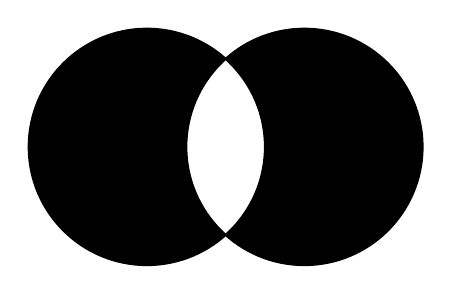
\begin{tikzpicture}[filled/.style={draw=black, fill=\fourthcolour, thick},outline/.style={draw=black, thick}]
	\draw[filled, even odd rule] (0,0) circle (1.5cm) node[xshift=-0.5cm] {$L(\mathcal{B})$}
							(0:2cm) circle (1.5cm) node[xshift=0.5cm] {$L(\mathcal{C})$};
\end{tikzpicture}
\caption{The symmetric difference of two languages $L(\mathcal{B})$ and $L(\mathcal{C})$}
\label{fig:symmetricdifference}
\end{figure}

The ``non-intersecting part" of two languages is more properly referred to as the \emph{symmetric difference} of the languages. Given two languages $L(\mathcal{B})$ and $L(\mathcal{C})$, their symmetric difference is the language
\begin{equation*}
L(\mathcal{B}) \symdiff L(\mathcal{C}) = \left( L(\mathcal{B}) \cap \overline{L(\mathcal{C})} \right) \cup \left( \overline{L(\mathcal{B})} \cap L(\mathcal{C}) \right).
\end{equation*}
The symmetric difference of $L(\mathcal{B})$ and $L(\mathcal{C})$ is illustrated by the shaded regions of the Venn diagram shown in Figure~\ref{fig:symmetricdifference}.

Since we know from earlier that the class of regular languages is closed under union, complement, and intersection, we can combine all of these closure properties to construct a deterministic finite automaton $\mathcal{D}$ whose language is $L(\mathcal{D}) = L(\mathcal{B}) \symdiff L(\mathcal{C})$. We will use this finite automaton $\mathcal{D}$ in our decision algorithm for the equivalence problem.

The idea behind this decision algorithm, as we mentioned before, is to test equivalence by testing the emptiness of the symmetric difference language. If $L(\mathcal{D})$ is empty, then we know that all words belong to the intersection of $L(\mathcal{B})$ and $L(\mathcal{C})$, and therefore $L(\mathcal{B}) = L(\mathcal{C})$.

\begin{theorem}\label{thm:EQDFAdecidable}
$\mathit{EQ}_{\DFA}$ is decidable.

\begin{proof}
Construct a Turing machine $\mathcal{M}_{\mathrm{EQDFA}}$ that takes as input $\langle \mathcal{B}, \mathcal{C} \rangle$, where $\mathcal{B}$ and $\mathcal{C}$ are deterministic finite automata, and performs the following steps:
\tmalgorithm{$\mathcal{M}_{\mathrm{EQDFA}}$}{
\begin{enumerate}
\item Construct a deterministic finite automaton $\mathcal{D}$ recognizing the language $L(\mathcal{D}) = L(\mathcal{B}) \symdiff L(\mathcal{C})$.
\item Run $\mathcal{M}_{\mathrm{EDFA}}$ from the proof of Theorem~\ref{thm:EDFAdecidable} on input $\langle \mathcal{D} \rangle$.
\item If $\mathcal{M}_{\mathrm{EDFA}}$ accepts, then accept. Otherwise, reject.
\end{enumerate}
}
This Turing machine accepts its input $\langle \mathcal{B}, \mathcal{C} \rangle$ if and only if $\mathcal{M}_{\mathrm{EDFA}}$ accepts its input $\langle \mathcal{D} \rangle$, where $\mathcal{D}$ is the deterministic finite automaton recognizing the symmetric difference language. This occurs only when the symmetric difference language is empty, and thus all of the words in both $L(\mathcal{B})$ and $L(\mathcal{C})$ appear in the intersection of these two languages; that is, $L(\mathcal{B}) = L(\mathcal{C})$. Likewise, the Turing machine rejects if and only if $\mathcal{M}_{\mathrm{EDFA}}$ rejects, which means that the symmetric difference language is nonempty and so $L(\mathcal{B}) \neq L(\mathcal{C})$. Since both the process of constructing $\mathcal{D}$ and the process of running $\mathcal{M}_{\mathrm{EDFA}}$ are finite, the Turing machine will never become trapped in an infinite computation. Thus, $\mathcal{M}_{\mathrm{EQDFA}}$ decides the equivalence problem for deterministic finite automata.
\end{proof}
\end{theorem}

Of course, we immediately have the usual corollary to accompany this result.

\begin{corollary}
$\mathit{EQ}_{\NFA}$ and $\mathit{EQ}_{\RE}$ are decidable.
\end{corollary}

\subsection*{Inclusion Problem}

\begin{construction}
Soon enough, we'll have a positive decidability result for the inclusion problem to go along with our collection of other positive decidability results.
\end{construction}